\documentclass[a0paper, portrait]{tikzposter}
\usepackage[utf8]{inputenc}

%%%%%%%%%%%%%%%%%%%%%%%%
%  table env for tkiz  %
%%%%%%%%%%%%%%%%%%%%%%%%
\newcounter{tablecounter}
\newenvironment{tikztable}[1][]{
  \def \rememberparameter{#1}
  \vspace{10pt}
  \refstepcounter{tablecounter}
  \begin{center}
  }{
    \ifx\rememberparameter\@empty
    \else
    \\[10pt]
    {\small Tab.~\thetablecounter: \rememberparameter}
    \fi
  \end{center}
}
%%%%%%%%%%%%%%%%%%%%%%
 
\title{The Genetic Architecure of Human Aggression}
\author{Robert M. Porsch}
\date{\today}
\institute{Center of Genomic Science}
%\titlegraphic{\includegraphics{1d.jpg}}
 
\usetheme{Simple}
 
\begin{document}
 
\maketitle

\block{Abstract}{ 
Aggression is the delivery of an aversive stimulus from one person to another with intent to cause harm.
Such behavior has potential beneficial and harmful consequences for the aggressor and can be seen to originate in the evolutionary principles of natural selection,
suggesting that genetic factors have a considerable impact on aggressive behavior.
Indeed, previous research has shown that about half of the variation of aggression can be explained by genetic factors.
However, it remains unknown to what extent these genetic effects differ across sex or overlap with factors affecting other phenotypes.
Furthermore, specific genetic loci associated with aggression remain unidentified. 

We have made use of a longitudinal sample of $17,662$ twin pairs (age 7 to 12) to explore the overall influence and stability of genetic factors on aggression, and their moderation by  age and sex  via structural equation models.
Furthermore, a genotyped sample of $152,247$ unrelated individuals (age 40 to 69) from the UK Biobank was used to identify specific genetic loci and to explore the genetic correlations across multiple traits related to aggressive behavior, namely smoking, neuroticism, alcohol consumption, and risk taking.
In addition a Mendelian randomization approach was applied to infer potential causal relationships between psychiatric disorders and aggressive behavior.

Twin models show high heritability (between 50\% and 80\%) and demonstrate stability of aggressive behavior across ages.
The analysis also suggested significant but small sex differences.
Furthermore, the stability of aggressive behavior is mainly driven by genetic factors.
Despite these high heritability estimates, no genome-wide significant association was identified.

Analysis of the genetic correlations with aggression showed high estimates for risk taking ($r_g=0.44$, $SE=0.103$), neuroticism ($r_g=0.63$, $SE=0.083$), and depression ($r_g=0.6741$, $SE=0.0919$).
Interestingly, while a Mendelian randomization approach suggests a causal effect of schizophrenia on both aggression and risk taking, a causal relationship between aggression and depression was not supported.

To conclude, these studies have helped to foster our understanding of the underlying genetic mechanisms of aggressive behavior.
Furthermore, it was shown that aggression is complex and genetically correlated with a number of other traits,
implying that future studies should consider  such behavior in conjunction with the related phenotypes.     
}

\begin{columns}
  \column{0.5}

    % Aim 
    \block{Aim}{
      \begin{itemize}
        \item Identification of \textbf{genetic loci} associated with impulsive Aggression and Risk Taking
        \item Investigate the \textbf{genetic overlap} between aggression and related phenotypes
        \item Explore \textbf{causal connection} among behavioral phenotypes
      \end{itemize}
    }

    % Methods and Samples
    \block{Methods}{
      \begin{itemize}
        \item Samples from the UK BioBank and publicly available summary statistics were used
        \item Heritability and Genetic Correlations were computed with LD-Score regression
        \item Potential causal pathways between psychiatric disorders and aggression/risk taking were investigated
      \end{itemize}
      \begin{tikztable}[Sample Size and Missingness of UK Biobank]
        \centering
        \input{tables/descriptive_ukb.tex}
      \end{tikztable}
    }

    % Genetic Correlation Matrix
    \block{Genetic Correlations}{
      \begin{tikzfigure}[Genetic Correlations within the UKB]
        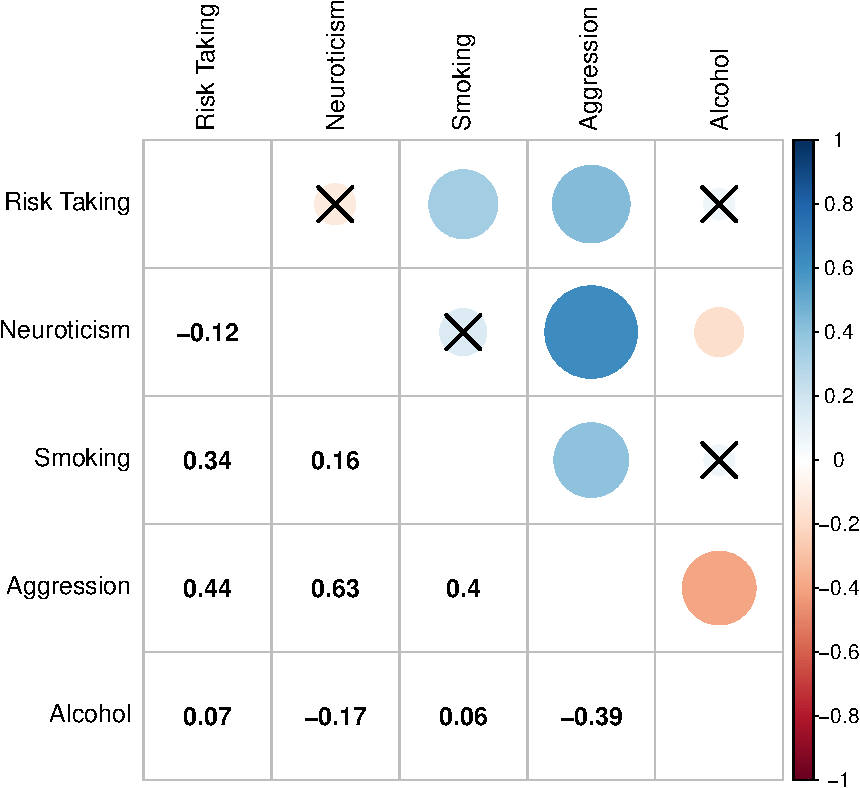
\includegraphics[width=0.65\linewidth]{../ukb_assoc/figure/genetic_corr/gcorr_plot_circle_full_se.pdf}
      \end{tikzfigure}
    }

    % Phenotypic Effects
    \block{Phenotypic Effects}{

      \begin{minipage}{0.49\linewidth}
        \begin{tikzfigure}[Phenotypic Correlations]
          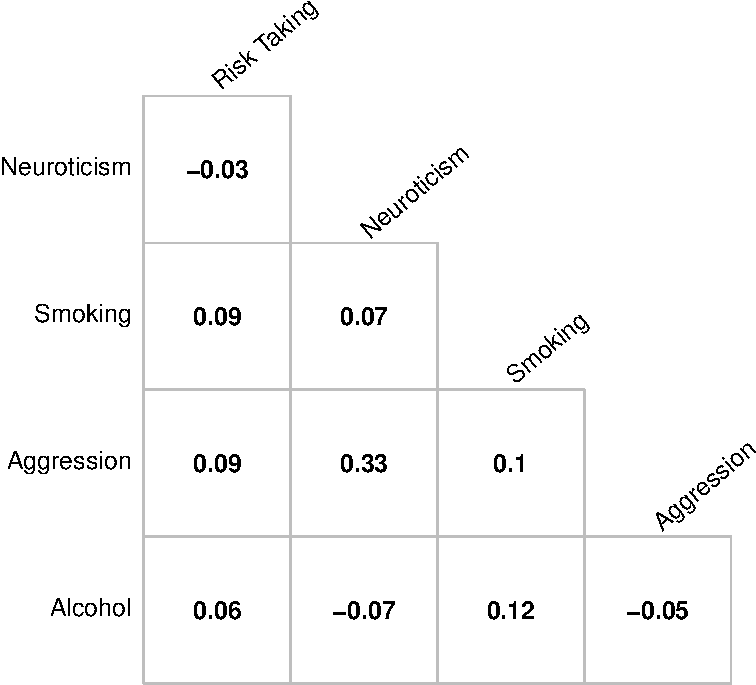
\includegraphics[width=0.99\linewidth]{../ukb_assoc/figure/phenotype/corr_plot_ci.pdf}
        \end{tikzfigure}
      \end{minipage} \hfill
      \begin{minipage}{0.49\linewidth}
        \begin{tikzfigure}[
          Effects of Age (A) and Sex (B) as well as the distrubition of Neuroticisim (C) and drinking behavior (D)
          ]
          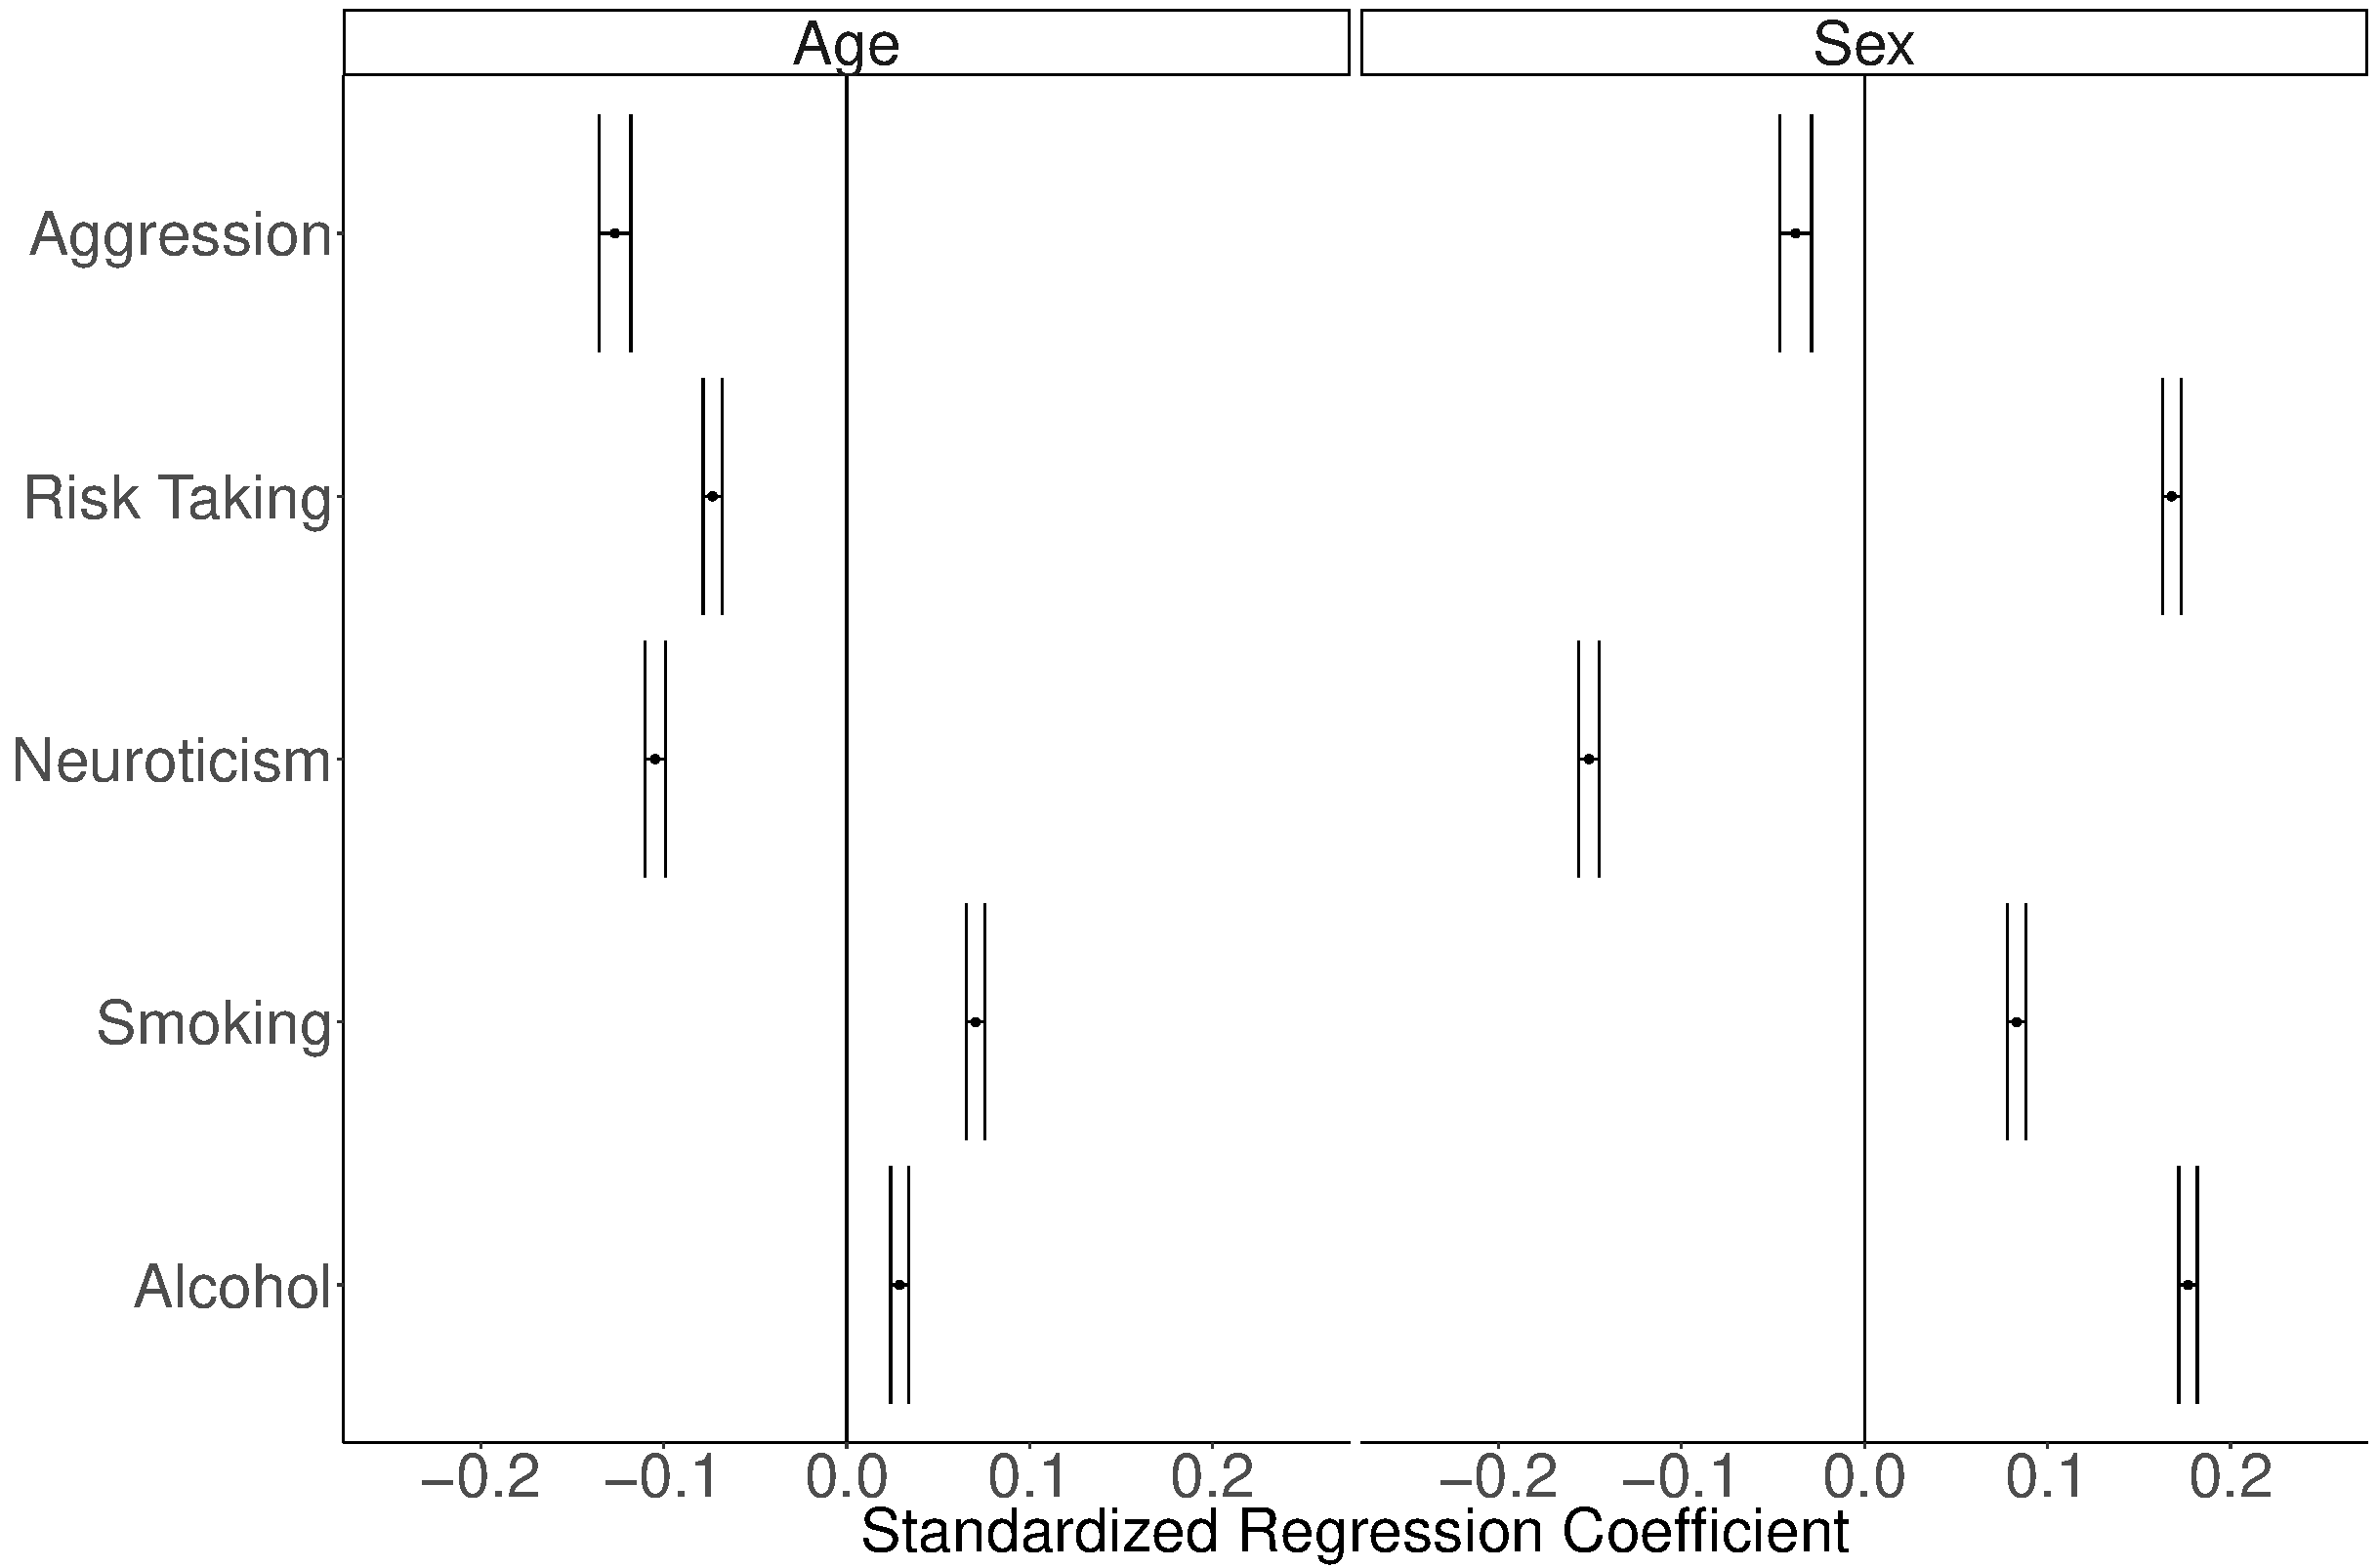
\includegraphics[width=0.99\linewidth]{../ukb_assoc/figure/phenotype/descriptives_plots.pdf}
        \end{tikzfigure}
      \end{minipage}
    }

  \column{0.5}

    % Association Results
    \block{Association Results}{
      \begin{itemize}
        \item Genome-wide significant signal in Risk taking but not Aggression
        \item Improved sample size or better phenotyping required
      \end{itemize}
      \begin{minipage}{0.49\linewidth}
        \begin{tikzfigure}
          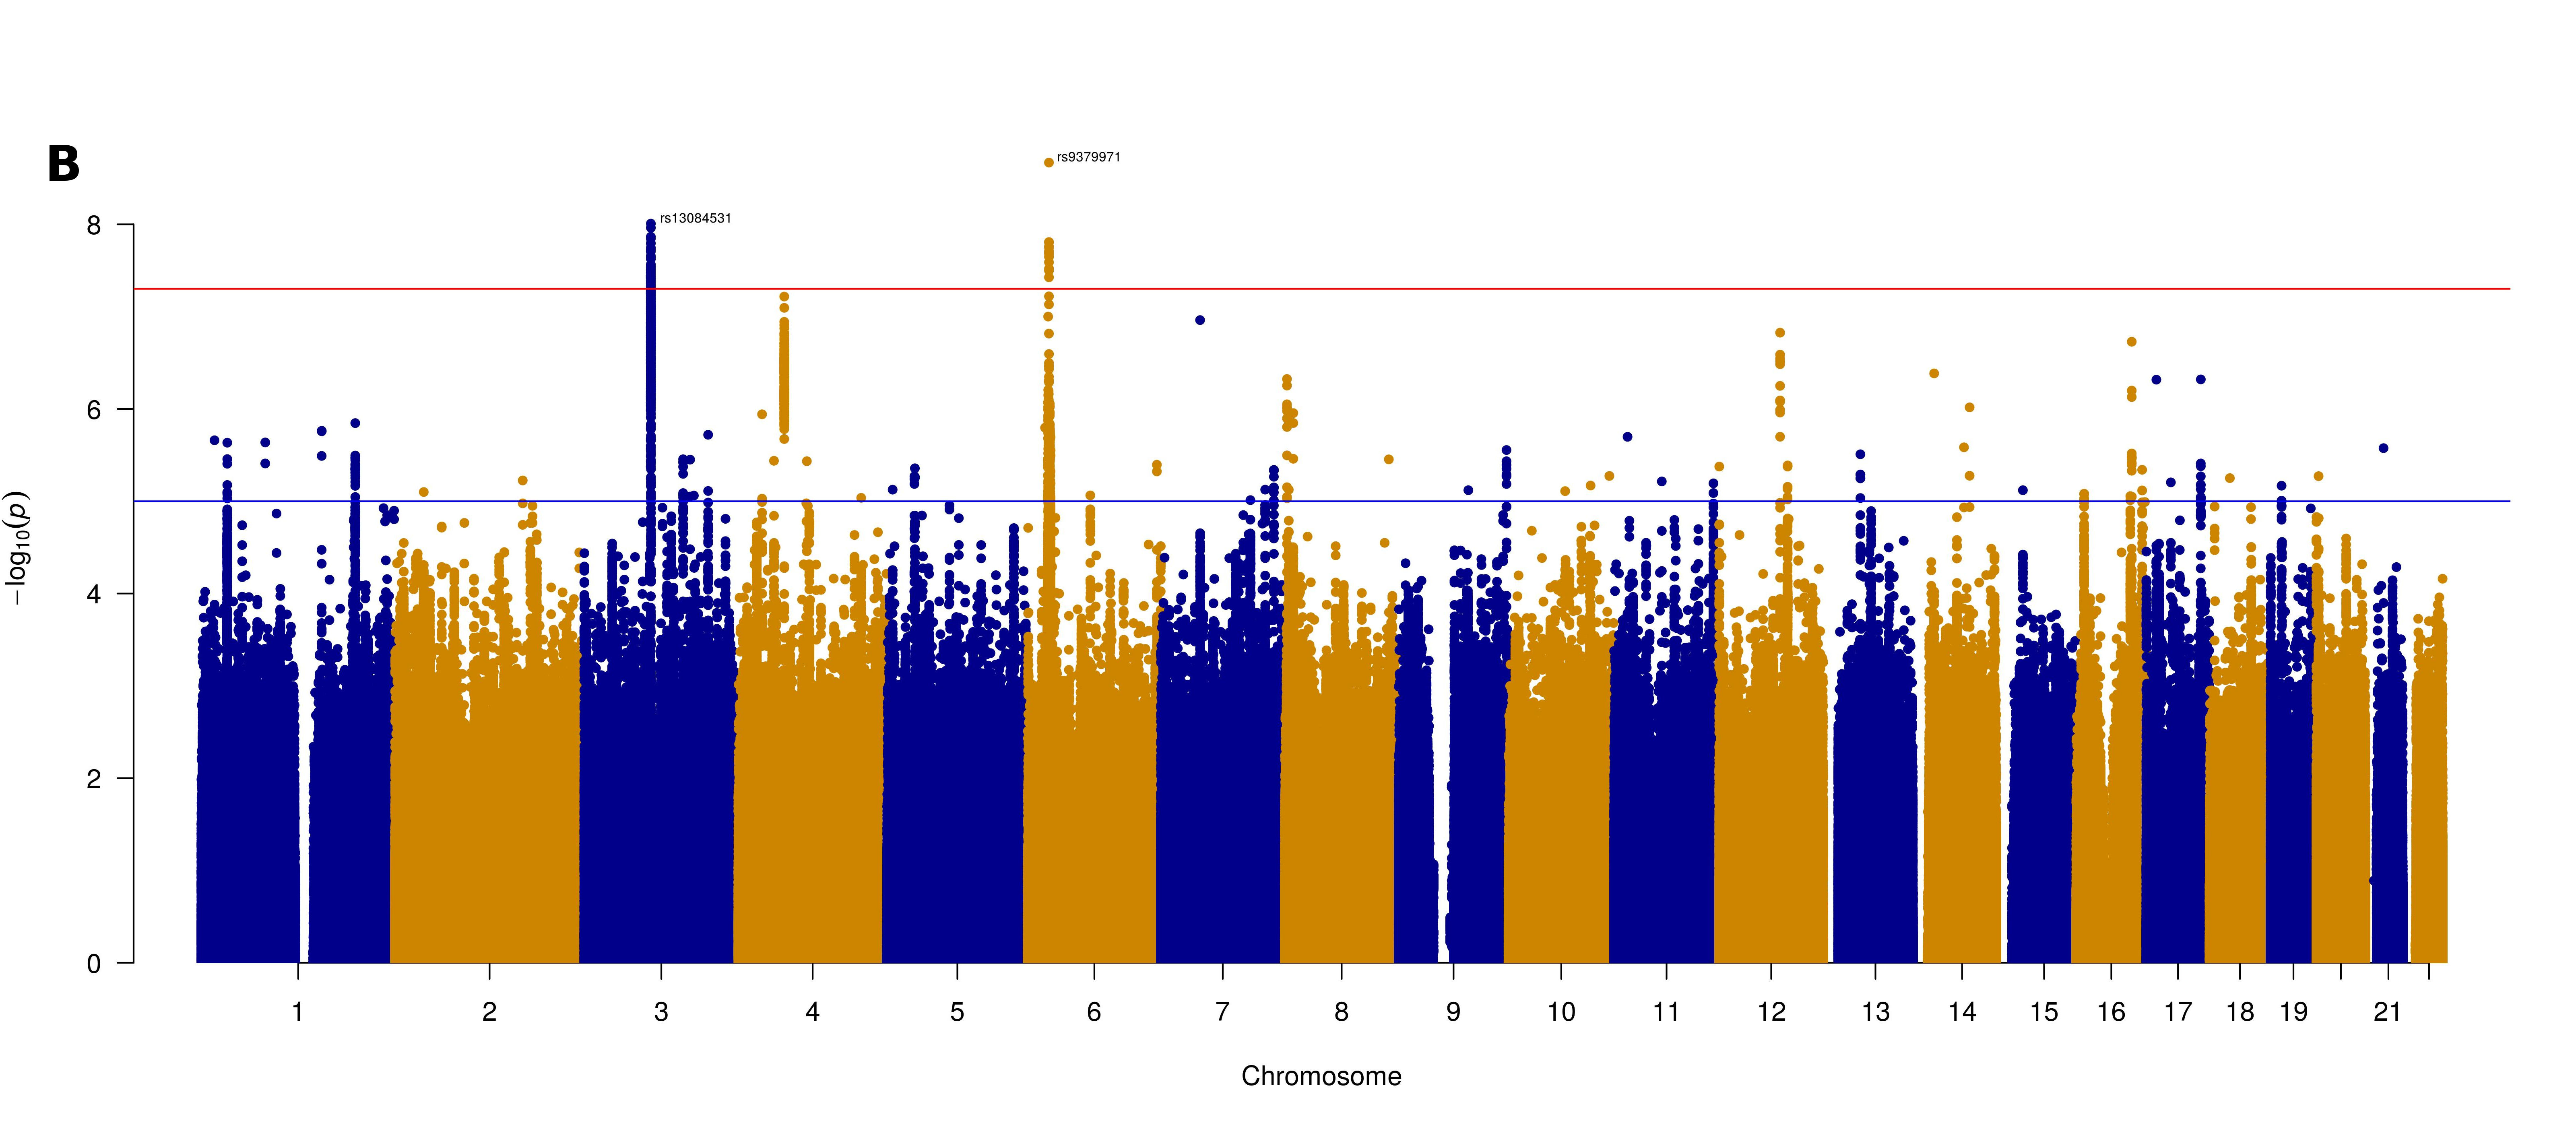
\includegraphics[width=0.8\linewidth]{../ukb_assoc/figure/manhatten_plots/risk_manhatten_color_B.jpeg}
        \end{tikzfigure}
      \end{minipage}
      \begin{minipage}{0.49\linewidth}
        \begin{tikzfigure}
          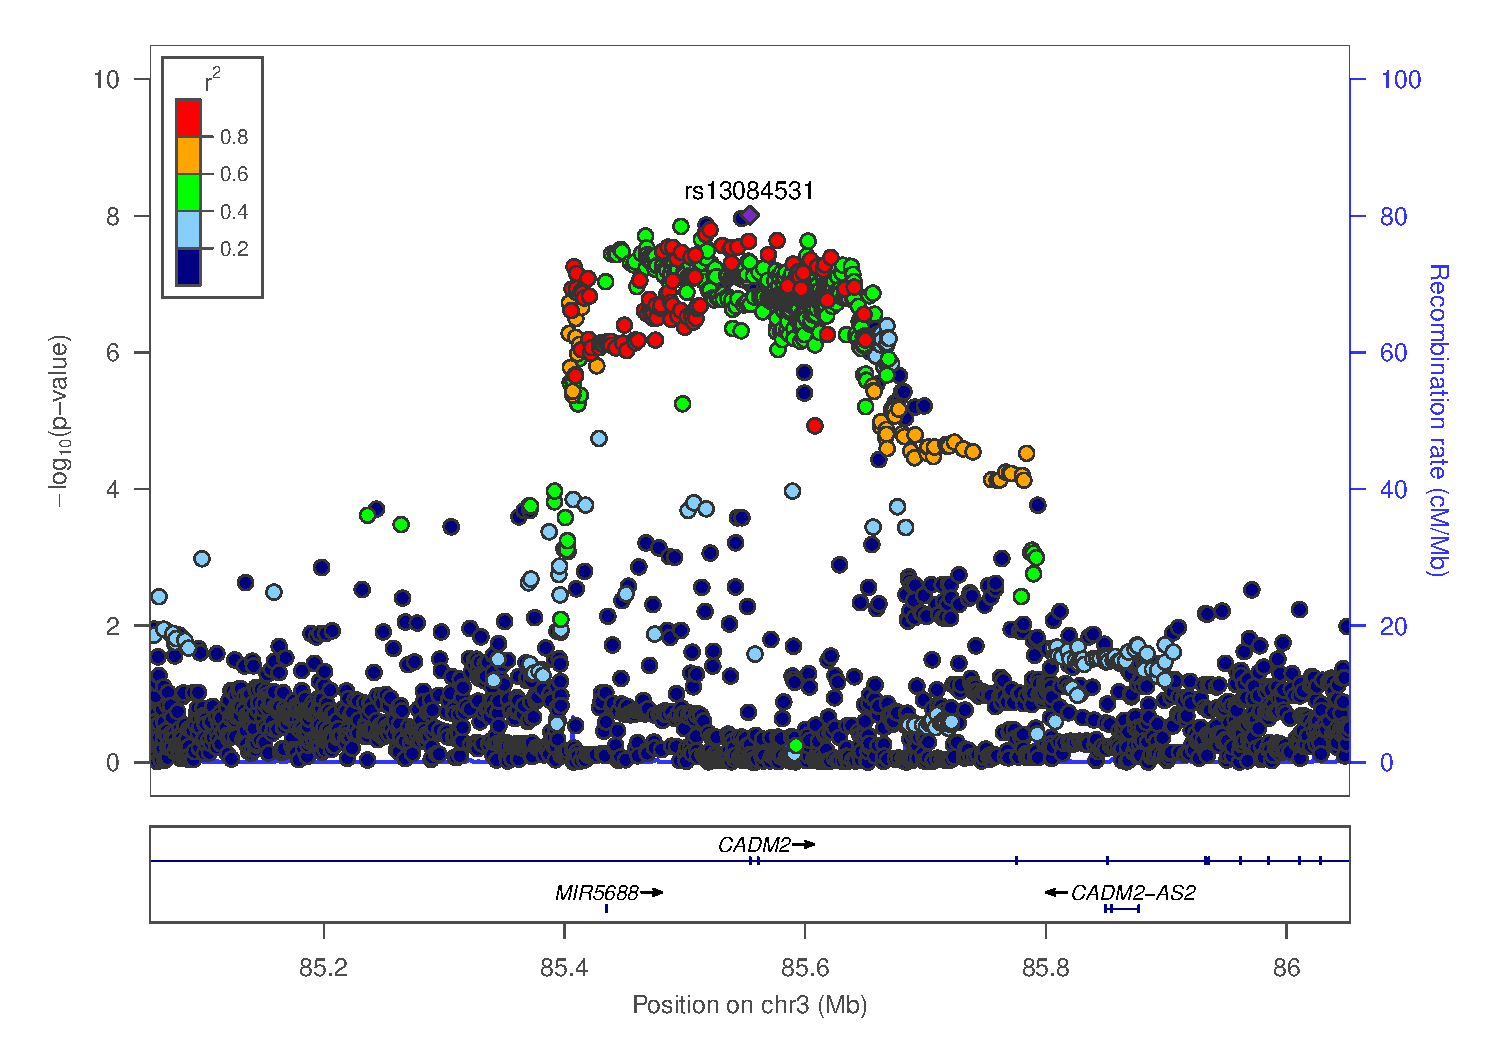
\includegraphics[width=0.7\linewidth, page=1]{{../ukb_assoc/figure/locuszoom/chr3_85055567-86052757}.pdf}
        \end{tikzfigure}
      \end{minipage}
    }

    % MR
    \block{Mendelian Randomization}{
      \begin{tikzfigure}[
        Estimated causal effect of psychiatric disorders on impulsive aggression and risk taking.
        The effect size of the causal effect $\beta$ is displayed on the y-axis, while used Mendelian randomization methods are on the x-axis.
        SZ, Schizophrenia; MDD, Major Depressive Disorder; DS, Depressive Symptom's; BP, Bipolar Disorder.
        (A) Effect of psychiatric disorders on impulsive aggression.
        (A) Effect of psychiatric disorders on risk taking.
        ]\label{fig:overall_mr_effect}
        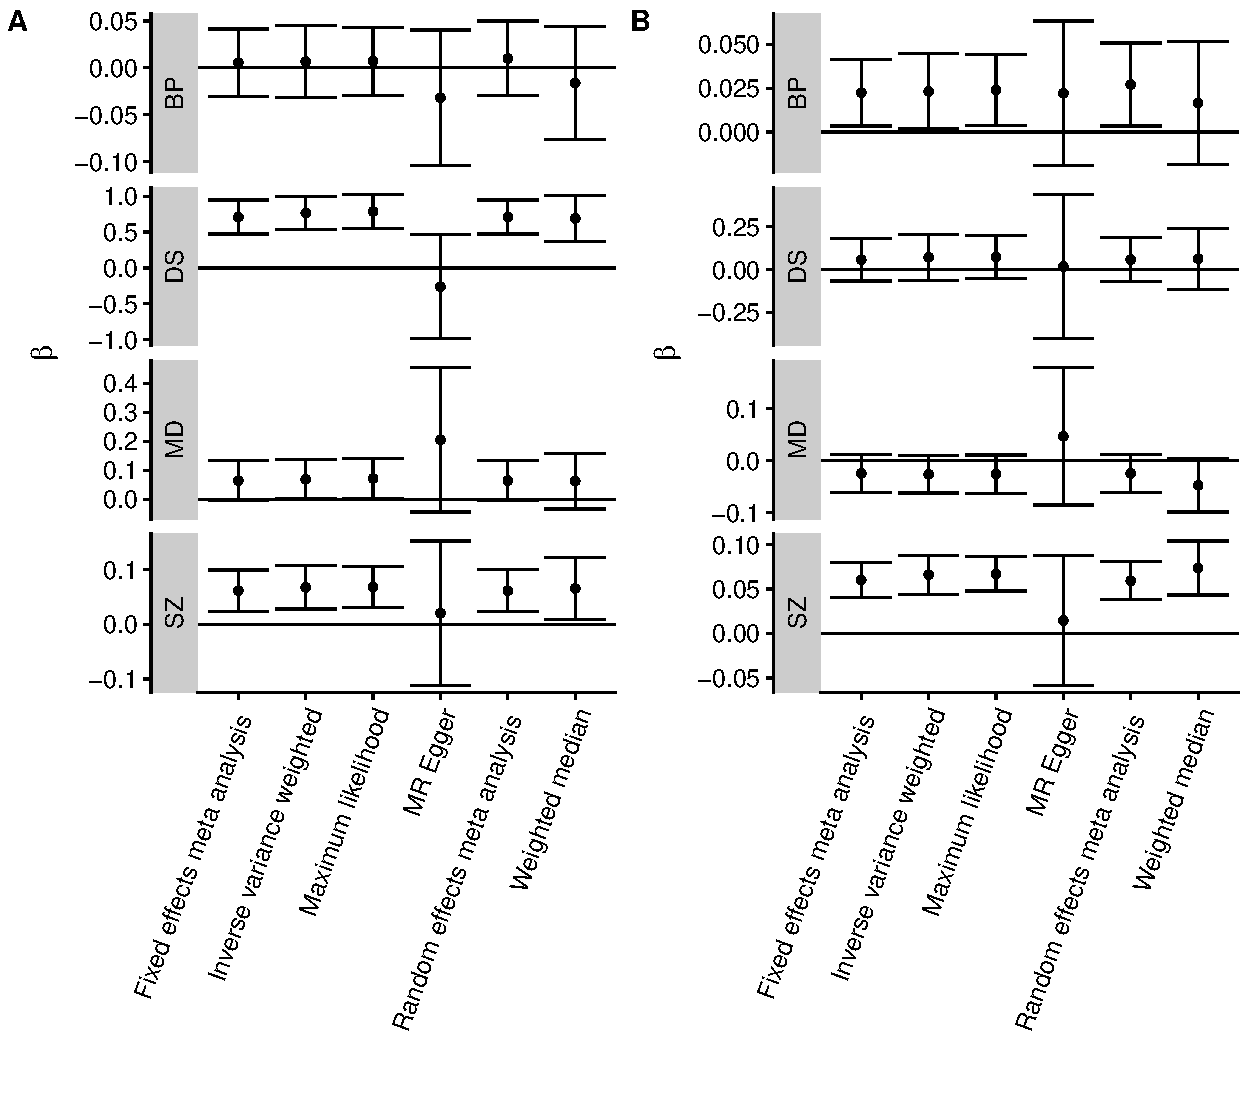
\includegraphics[width=0.6\linewidth]{../ukb_psychiatric/figures/overall_mr_effect.pdf}
      \end{tikzfigure}

      \begin{itemize}
        \item Estimated causal effects are small
        \item Some indication for a causal connection betwee SZ and aggression/risk taking
      \end{itemize}

      \begin{tikzfigure}[Sensitivity analysis.
        (A) Displays the intercept $\beta_0$ of MR-Egger regression for psychiatric disorders on impulsive aggression. The intercept is an indication of whether directional horizontal pleiotropy is driving the MR analysis.
        (B) The MR-Egger regression intercept of psychiatric disorders on risk taking.
        (C) Funnel plot of Depressive symptoms on impulsive aggression. 
        (D) Funnel plot of MDD on impulsive aggression. 
        (E) Funnel plot of SZ on impulsive aggression. 
        (F) Funnel plot of SZ on risk taking. 
        The intercept of both MR-Egger and Inverse variance method are indicated with a vertical line.
        Error bars indicate the 95 confidence intervals.
        ]\label{fig:sensitivity}
        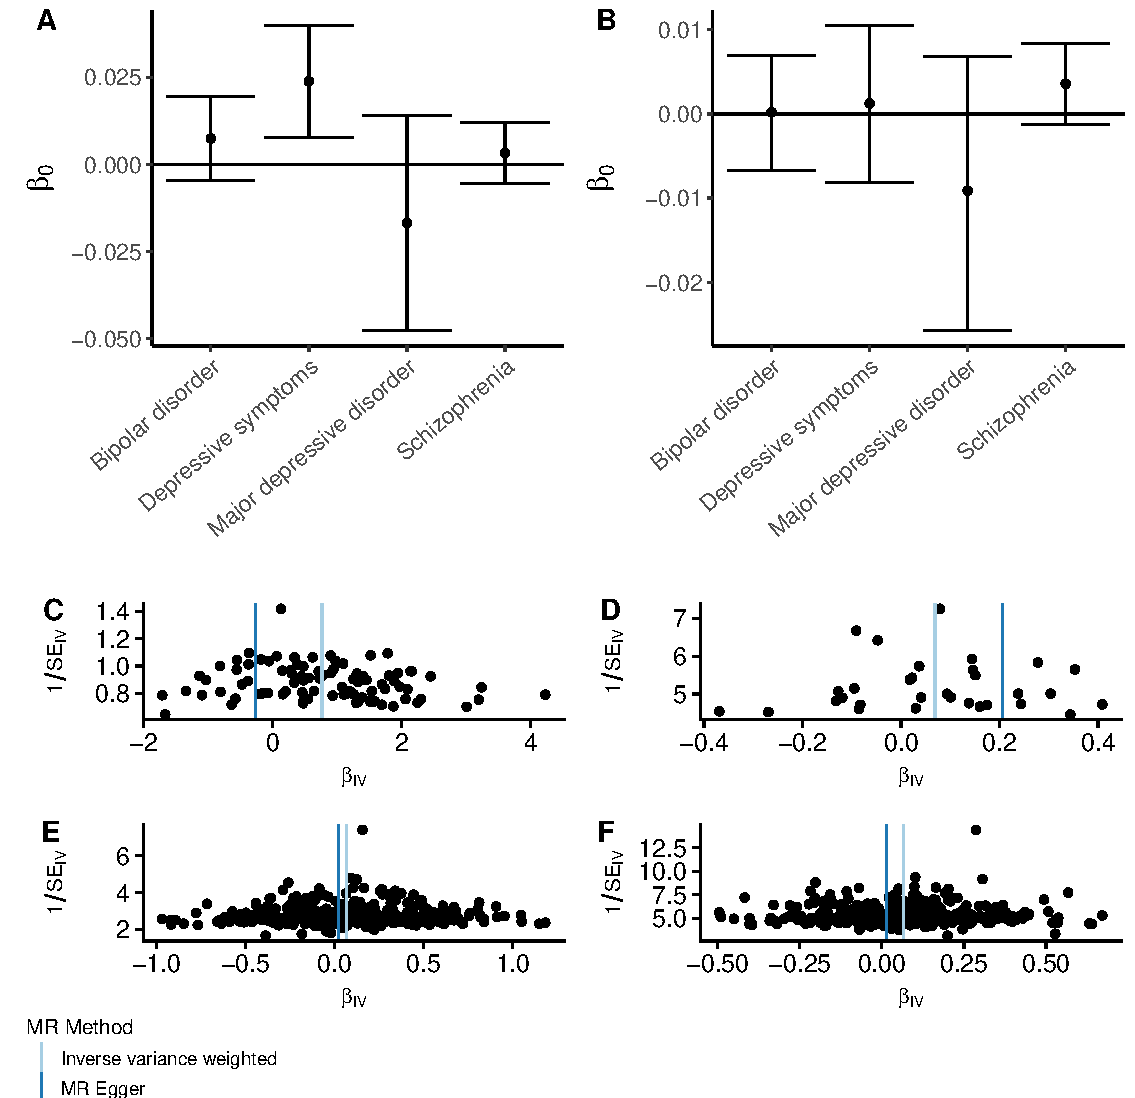
\includegraphics[width=0.6\linewidth]{../ukb_psychiatric/figures/sensitvity_plot.pdf}
      \end{tikzfigure}
    }

\end{columns}

\end{document}
